\section{M = 4--5 D}
\begin{center}
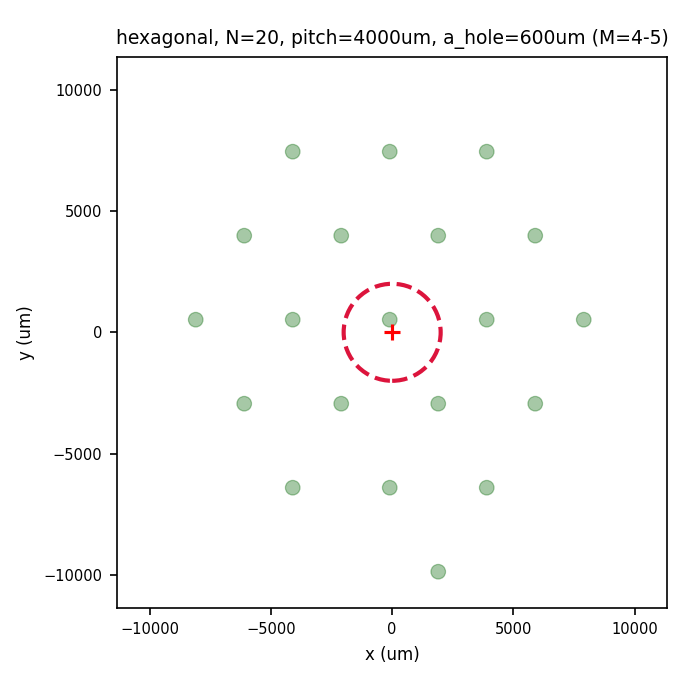
\includegraphics[width=0.55\textwidth]{gaze_weighted_viz_figs/fig_M4_5.png}
\end{center}
\texttt{hexagonal}, pitch=4000\,$\mu$m, N=20, a\_hole=600\,$\mu$m.
0.00\%/0.00\%.

\section{M = 6 D, M = 8 D}
\begin{center}
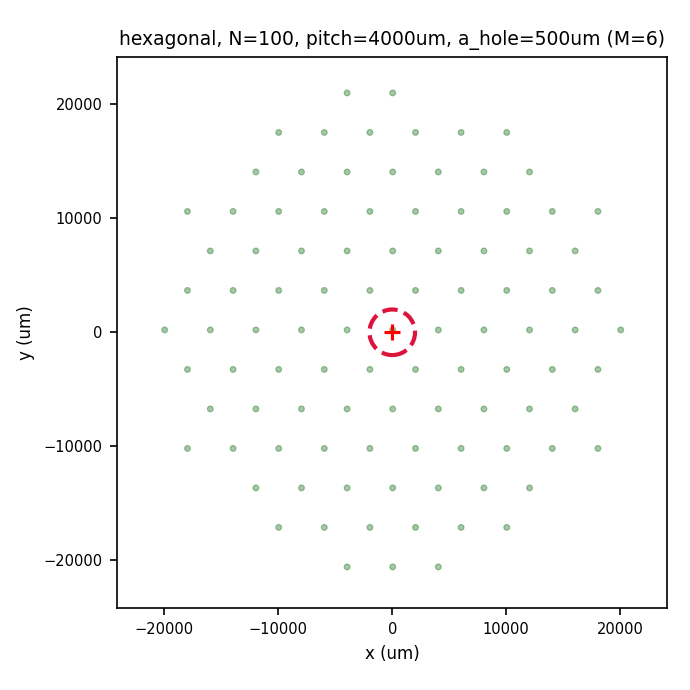
\includegraphics[width=0.48\textwidth]{gaze_weighted_viz_figs/fig_M6.png}\quad
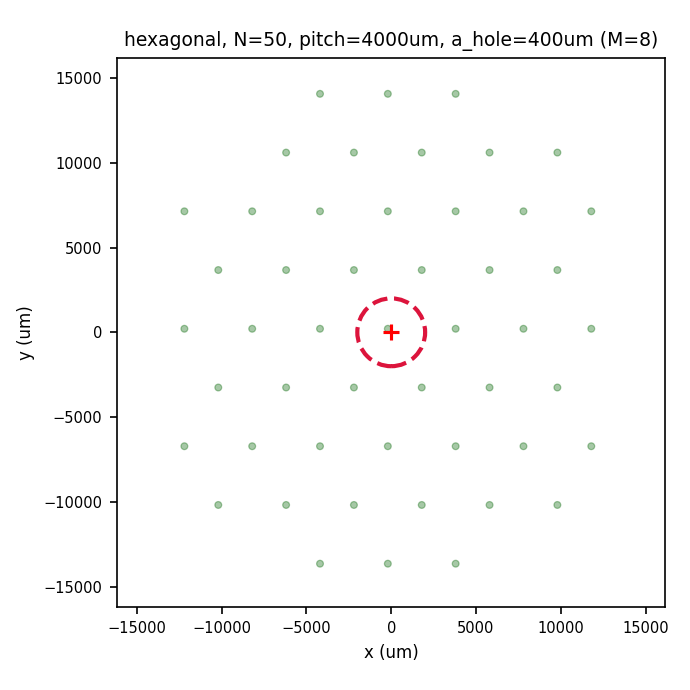
\includegraphics[width=0.48\textwidth]{gaze_weighted_viz_figs/fig_M8.png}
\end{center}
\texttt{hexagonal}, N=100 (M=6, left) and N=50 (M=8, right), same pitch and
family. These are the only two designs in the set with nonzero blind rate
(0.12\% and 0.33\%) --- still ghost-free, and both blind percentages are
smaller than the smallest nonzero value in the worst-case-optimal table.

\newpage
